\subsection{Menus}
	\subsubsection{API et widget}
	\paragraph{Android\\}
		Afin de créer les différents menus de notre application, Android met à la
		disposition des developpeurs une API\footnote{API : Application Programming
		Interface, c'est un ensemble de classes mis à disposition par une
		bibliothèque logicielle.} très bien fournie. Parmis celle-ci le package Widget
		nous a été très utile. 
		
		Grâce à ce dernier de nombreux objets ont été utilisé
		afin de mettre en oeuvre et rendre pleinement fonctionnel nos menus.
		Parmi les plus utilisés il y a eu bien sûr Button, TextView, CheckBox et
		EditText pour les plus explicites. Les objets comme Spinner, SeekBar et
		Gallery étant respectivement utilisés pour les menus déroulants, les barres de
		progression et les galeries d'images pour la sélection de cartes de jeu.
		
		Les composants graphiques sont créés ici au travers du fichier déclaratif
		XML via une synthaxe bien particulière. Cette méthode est vraisemblablement
		préférable, du moins lorsque l’interface graphique est figée, connue à l’avance. 
		Exemple :
		\begin{verbatim}
		
		<Spinner android:layout_width="wrap_content"
				 android:layout_height="wrap_content"
				 android:id="@+id/accounts"
				 android:layout_gravity="center_horizontal"
				 android:prompt="@string/ChooseUserAccount"></Spinner>
				
		\end{verbatim}		
		
		
		Pour récupérer la référence d’un widget créé depuis le
		fichier xml de layout, il convient d’utiliser la méthode findViewById de la
		classe Activity dans nos classes Java.
		
		Exemple :
		\begin{verbatim}
			Spinner sp = (Spinner)findViewById(R.id.accounts);
		\end{verbatim}
		
		On peut remarquer que cette méthode accepte en paramètre un int et non un
		String comme on pourrait s’y attendre. En effet, l’id est exprimé sous forme de constante int, on
		ne passe pas à la méthode la chaîne de caractères proprement dite. Grâce à cela, la
		méthode est sûre et on évite ainsi les erreurs à l’exécution qu’on pourrait avoir si on
		spécifiait un id ne correspondant à aucun widget.
		
		Concernant leur positionnement, un système de layout est utilisé. Les layouts sont des ViewGroup responsables
		du dimensionnement et du positionnement des widgets à l’écran. Il en existe plusieurs, 
		chacun adoptant une stratégie bien spécifique. 
		
		En ce qui nous concerne nous avons principalement utilisé les
		\textit{ListView, LinearLayout, TableLayout} et enfin les \textit{RelativeLayout}. Ce dernier nous a été très utile. En
		effet les widgets contenus dans un RelativeLayout peuvent déclarer leur position relativement
		par rapport à leur parent ou par rapport aux autres widgets. De ce fait nos
		menus et autres interfaces graphiques conservent leur proportion et leur
		agencement originel.		
		
		
		Les listeners présents dans	les classes java permettent à leur tour d'écouter les évènements utilisateurs
		ou system et réagir en fonction comme l'accès au menu suivant ou le lancement
		d'un partie. 
		
		
		Les activités sont des composants centraux des applications. Ce sont également les
		composants qui portent les éléments visuels de l’interface utilisateur agencés
		sur l’écran. La navigation entre les écrans se fait dans notre cas de façon
		explicite. L’ordre de changement d’activité est véhiculé par un objet de type Intent (intention en anglais).
		Les activités s’enchaînent les unes aux autres par invocation directe.
		C’est-à-dire qu’une activité donnée déclenche l’affichage d’une autre activité 
		en appelant la méthode startActivity avec un Intent mentionnant clairement le nom
		de l’activité. 
		
		Voici un exemple représentant la cohabitation listener Activity:
		
		\begin{verbatim}
		private Button create;
		this.create = (Button)findViewById(R.id.SinglePlayerGame);
		this.create.setOnClickListener(this);
			
		public void onClick(View view) {
		       Intent intent = null;
		       if( view == create ){
		             intent = new Intent(SinglePlayer.this, SinglePlayerLayout.class);
		             startActivity(intent);
		             this.finish();
		       }
		}
		\end{verbatim}
		
		
		
		
		
		
	\paragraph{iOS\\}
		
		Comme Android, nous avons utilisé les widgets \footnote{Widget est un élément de base d'une interface graphique  avec lequel un utilisateur peut interagir  (par exemple : une fenêtre, une zone de texte, un bouton, etc).} pour réaliser notre interface graphique. iOS fournit lui aussi une API couplet à une documentation très complète facilitant la réalisation d'une interface utilisateur ergonomique. Parmi les widgets les plus utile, nous retrouvons les UIView, UITableView, UITableViewCell, UILabel, UITextField, UIButton qui permettent respectivement de créer une vue, un tableau, une cellule du tableau, des labels, des champs de texte et des boutons.
	
	Pour manipuler ces différentes composant graphique, il est possible et beaucoup plus pratique d'uliser Interface Builder pour réaliser des menus. Interface builder permet de gagner du temps lors de la réalisation d'une interface graphique standard (de type menu). Cette réalisation est possible via un outil visuel et non des lignes de code,  Interface Builder va créer des fichiers xib \footnote{xib est l'acronyme de Xml Interface Buillder.} qui vont générer à la compilation des fichiers nib \footnote{nib es l'acronyme de NeXT Interface Builder.}. Ce dernier stock les informations relative à l'interface sous forme d'un fichier xml, mais nous avons pas besion de savoir réellemet comme ça fonctionne car il est inutile de modifier directement le fichier xml.
	
	Ensuite pour controller les différents l'élements de l'interface préalablement créées avec Interface Builder, il suiffit de les lier au code de la vue via ce dernier. Grâce a ces liaisons, il nous sera possible de les modifiers ou les controllers avec du code et donc de pouvoir les accorder avec les données du modèle.
	
	La gestion des écouteurs se fait grâce au même procédé qui est utilisé pour lier les éléments de l'interface avec la vue sauf que ça créra une métohde au lieu de créer un champs. Voilà un exemple d'écouteur :
	
	\begin{verbatim}
		- (void)playerAction:(id)sender {
		    if (sender == playerWhite) {
		        self.editorInformation.colorPlayer = @"white";
		    }
		    else if (sender == playerBlue) {
		        self.editorInformation.colorPlayer = @"blue";
		    }
		    else if (sender == playerRed) {
		        self.editorInformation.colorPlayer = @"red";
		    }
		    else if (sender == playerBlack) {
		        self.editorInformation.colorPlayer = @"black";
		    }
    
		    [editorInformation changeTool:@"player"];
		}
	\end{verbatim}
	
	Pour finir, l'un des principaux point de la gestion de l'interface graphique repose sur le modèle MVC et donc chaque vue doit être associée à un controlleur.
				
	\subsubsection{Première utilisation}
	\subsubsection{Création utilisateur}
	\subsubsection{Gestion utilisateur}
	\subsubsection{Gestion des préférences système}
	\subsubsection{Création de carte (charger)}
	\subsubsection{Création partie solo (tout)}
	\subsubsection{Création partie multi (officielle)}
			

\subsection{Editeur de carte}

	\hypertarget{Editeur de carte}{}
	\label{Editeur de carte}

	\subsubsection{Le modèle}
		La carte est la principale information que l'éditeur de carte doit gérer. Pour représenter une carte, nous avons choisi de la représenter sous la forme de deux matrices ayant les mêmes dimensions que la carte. La première matrice contient des \textit{Objects} représentant le sol et la deusième contient elle aussi des \textit{Objects} mais ces derniers représentent des blocs et non le sol. Pour gérer les deux matrice nous avons utilisé des \textit{NSMutableArray} qui sont des tableaux Objective-C que l'on peut modifier, ils contiennent eux aussi des \textit{NSMutableArray} car il n'existe pas des constructeurs de matrice comme en JAVA. Ensuite l'autre information que la carte doit possèder c'est la position de départ des joueurs. Nous avons utilisé un \textit{NSMutableDictionary} permettant de faire la liaison entre la couleur du joueur et son point de départ. 
			
		Lorsque l'utilisateur à terminé de créer ça carte, il a besoin de la sauvegarder. Pour cela nous avons donc utilisé la sérialisation des objets et lors de l'enregistrement de la carte ça génère un fichier \og .klob \fg \, qui contiendra les informations necessaires pour la reconstruction de la carte lors de son chargement qui la reconstruira en la déserialisant. Pour utiliser la serialisation en Objective-C, nous avons juste besoin implémenter le protocol \textit{NSCoding} qui comporte deux methode à définir : 
		\textit{- (id)initWithCoder:(NSCoder *)aDecoder} permettant de déserialisé et \textit{- (void)encodeWithCoder:(NSCoder *)aCoder} s'occupant de la serialisation.
	
	\subsubsection{La vue}
		Pour facilité le développement mais aussi ça réutilisabilité, nous avons découpé la vue de l'éditeur de carte en trois zones. Chaqu'une de ces vues est associée à un controlleur qui permettra de faire la liaison avec le modèle. Pour concevoir les vues nous avons utilisé la classe UIView qui est prévue pour réaliser des vues pour une interface graphique sur iPhone. 
			
		\begin{center}
			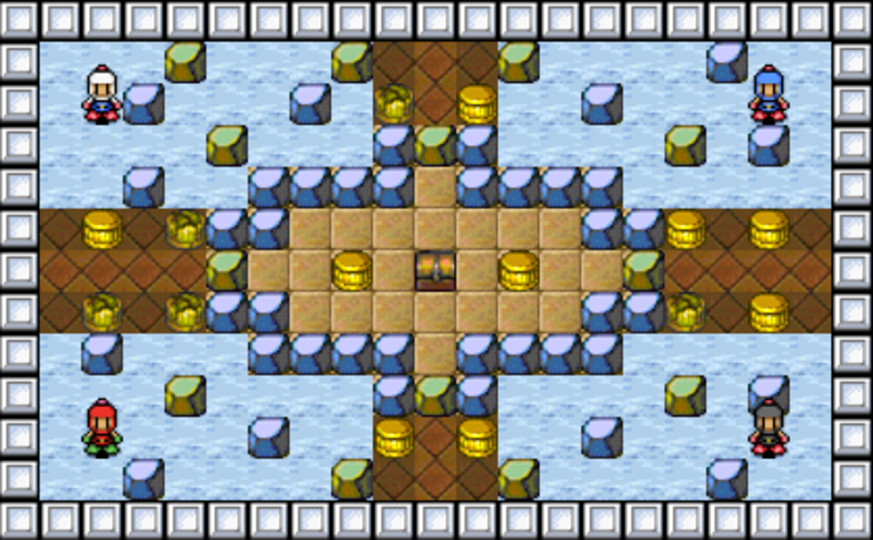
\includegraphics[width=11cm]{./Developpement/Img/carte.pdf}
		\end{center}
		Tout d'abord, la vue la plus important que nous avons créé, c'est la vue affichant la carte permettant au joueur d'intéragir avec celle-ci et de pouvoir créer des cartes selon ses envies. Pour réaliser cette intéraction, nous avons dû surcharger trois methodes de la classe \textit{UIResponder} : \textit{touchesBegan}, \textit{touchesMoved} et \textit{touchesEnded} permettant de gérer tous les évènement générés lorsque l'utilisateur appuiera sur la vue. La methode \textit{touchesBegan} permet de récupérer l'évènement lorsque l'utilisateur va appuyer sur la vue, grâce à cette évènement, on peut savoir à quelle position l'utilisateur à pressé la vue. Ensuite pour réccupérer l'évènement lorsque l'utilisateur continu d'appuyer sur l'écran, il nous suffit d'utiliser \textit{touchesMoved}. Et pour finir lorsque l'utilisateur retire son doigt de la vue, nous utilisons la méthode \textit{touchesEnded} qui nous permettra par exemple de savoir où l'utilisateur à retiré son doigt de la vue. A l'aide de ces trois methodes, nous avons implémenté les différents gestes que l'ulisateur peut effectuer pour créer une carte. Pour dessiner la carte, nous avons dû surcharger la methode \textit{- (void)draw:(CGContextRef)context}, celle-ci permet de modifier le comportement de l'affichage de la vue et notamme elle donne la possibilité de dessiner n'import quel objet dans la vue.
		
		\begin{center}
			
\includegraphics{./Developpement/Img/menu_droite.pdf}
		\end{center}
			
		Ensuite, nous avons créer une vue permettant de changer d'objet que l'on veut mettre sur la carte. Cette dernière se trouve à gauche de la carte. Dans cette vue, nous avons des \textit{UIButton} permettant de créer des boutons, mais la partie la plus important de la vue c'est la liste déroulante pour choisir l'objet que l'on placer sur la carte. Cette liste déroulante est une vue que nous avons dû implémenter, la particularité de cette liste c'est qu'elle est générique ce qui permet de l'utiliser dans plusieurs vues différentes et notamment dans les menus pour afficher le choix des cartes. Grâce à celle-ci l'utilisateur peut changer d'objet selectionné en exerçant un simple mouvement vertical du doigt.
			
		\begin{center}
			
\includegraphics[width=11cm]{./Developpement/Img/menu_haut.pdf}
		\end{center}
		Enfin la dernière vue que nous avons réalisé, est une vue contenant plusieurs \textit{UIButton} mais aussi un \textit{UISegmentedControl} qui permet de basculer du mode affichage complet (dessiner tous les éléments de la carte) de la carte, au mode d'affichage partiel (qui affiche que le sol et cache les blocs de la carte) facilitant la modification du sol malgrès les blocs.
			
			
	\subsubsection{Le controlleur}
		
		Le controlleur est une partie très important de l'architecture MVC, elle permet de faire le lien en les interactions que l'utilisateur effectue dans l'éditeur de carte et les données relative à celui-ci. Nous avons  donc créé des objets de type \textit{UIViewControler}, ces objets nous ont permis de réaliser cette liason. Grâce à celle-ci, le modèle et la vue sont complètement indépend ce qui permet de pouvoir changer totalement de vue sans avoir besoin de modifier le modèle. Comme nous avons divisé l'éditeur de carte en plusieurs sous vues, nous avons donc créé un \og pseudo \fg controlleur (car se ne sont pas des \textit{UIViewControler} mais seulement des objets normaux) pour chaqu'une entre elles, elle même possède un controlleur global qui lui sera bien un \textit{UIViewControler}. Lorsqu'un utilisateur va réaliser une action dans la vue de l'éditeur de carte, cette dernière va appeler une methode de son pseudo controleur, qui lui appelera une methode du controlleur global, qui se chargera d'appeler la bonne methode du modèle en fonction de l'action effectuée par l'utilisateur. 



\subsection{Jeu}

	\subsubsection{Moteurs}
	
		Au sein d'un jeu vidéo plusieurs types de moteurs sont mis en place.
		Chacun a un travail bien précis.
		Ici nous en retrouvons trois au total à savoir un pour le rendu graphique, un
		pour s'occuper de la physique et un dernier gerant les actions de
		l'intelligence artificielle.
		Commencons par le moteur de rendu.
	
		\paragraph{Moteur de rendu\\}
		
			\hypertarget{Moteur de rendu}{}
			\label{Moteur de rendu}
		
			Contrairement à celui que nous avons vu dans la section précédente pour
			l'éditeur de carte
			\footnote{
				\hyperlink{Editeur de carte}{Editeur de carte}
				\og voir section \ref{Editeur de carte}, page \pageref{Editeur de carte}.\fg
			}
			le moteur de rendu se doit être beaucoup plus léger car le jeu doit dans son
			ensemble rester le plus fluide afin d'offrir à l'utilisateur une meilleure
			experience vu qu'ici il faut en plus de gérer le rendu, s'occuper du
			physique
			\footnote{
				\hyperlink{Moteur physique}{Moteur physique}
				\og voir section \ref{Moteur physique}, page \pageref{Moteur physique}.\fg
			}.
			, de l'intelligence artificielle
			\footnote{
				\hyperlink{IA}{IA}
				\og voir section \ref{IA}, page \pageref{IA}.\fg
			}.
			et des divers sons
			\footnote{
				\hyperlink{Sons}{Sons}
				\og voir section \ref{Sons}, page \pageref{Sons}.\fg
			}.
			qui seront joués au cours de la partie.		
			
			$\,$	
			
			L'utilisateur ne pourra plus modifier la carte à sa guise et sera
			entièrement dépendant du moteur physique\footnotemark[3] c'est à dire par
			exemple qu'ici un bloc indestructible sera présent tout au long de la
			partie et ne pourra pas être supprimé, il n'est donc plus necessaire de
			savoir quel type de sol se trouve dessous, de plus comme celui-ci ne peut pas
			être détruit et qu'il n'est pas animé son état sera toujours le même et ne
			correspondra qu'à une seule et unique image.
			
			$\,$			
			
			Un autre exemple est celui d'un sol inanimé tel que l'herbe où si il n'y a
			aucun bloc (destructible) au dessus en début de partie il en sera de même à
			la fin donc il ne nous est pas necessaire à chaque rafraichissement de
			regarder si un bloc existe dessus, ce test se fait en début de partie est
			sera valide jusqu'à la fin de celle-ci.
			
			
			Cette remarque s'applique sur tous les objets dits \emph{non animés} dont
			l'état ne changera jamais au cours du jeu et seulement eux.
			
			
			Si l'on avait eu un sol animé représentant de l'eau, il aurait été composé de
			plusieurs images et aurait donc necessité un rafraichissement constant.

			$\,$
			
			Concrètement ce que nous faisons ici à chaque début de partie est de créer
			une image vierge qui aura la taille de la carte affichée sur l'écran dans
			laquelle nous dessinerons tous les objets \emph{non animés}.
			
			$\,$
			
			Pour cela nous allons parcourir les deux matrices définies dans l'éditeur de
			cartes\footnotemark[2] et regarder s'il existe un bloc, si oui est-ce
			qu'il est destructible ?
			
			Si ce bloc est destructible alors il nous est obligatoire de savoir ce qui se
			trouve en dessous.
			Nous allons donc stocker ce bloc dans une hashmap dont les cléfs sont les
			coordonnées de l'objet et dont la valeur est l'objet lui même et dessiner le
			sol sur l'image citée au dessus.
			
			Si ce bloc est indestructible alors inutile de mémorisé le sol se trouvant
			au dessous.
			
			Sinon s'il n'existe pas de bloc nous allons regarder si le sol est animé, si
			oui alors nous le stockons dans la hashmap comme un bloc destructible sinon
			nous le dessinons dans l'image comme un objet inanimé.
			
			$\,$
			
			Voici un exemple concret de la methode décrite au dessus :
				

			\begin{figure}[!h]			
				\begin{center}			
					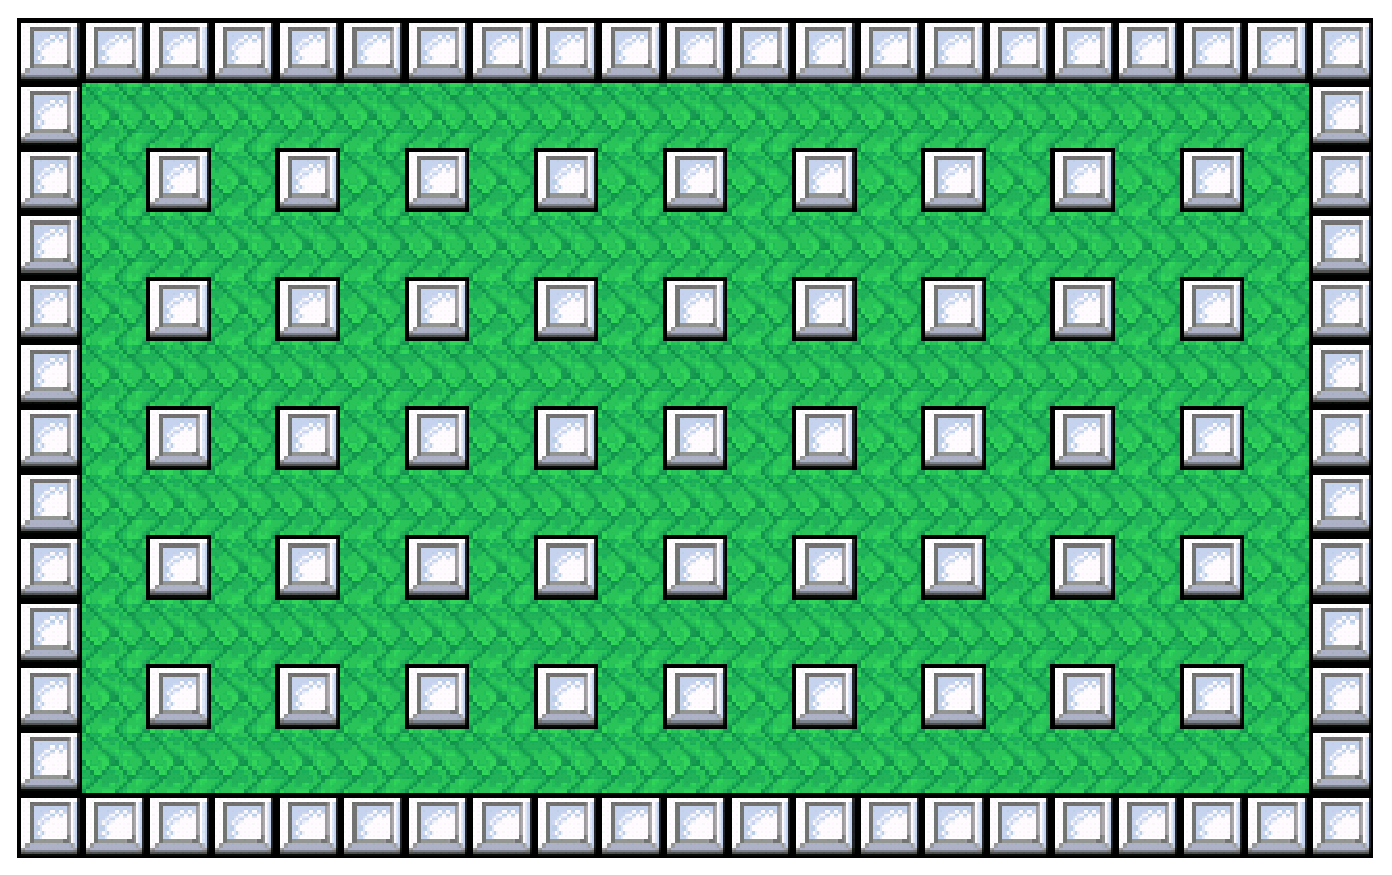
\includegraphics[width=229px, height=142px]{Developpement/Img/map.eps}
					\caption{L'image représentant la totalité des objets non animés}
				\end{center}
			\end{figure}
			
			$\,$			

			\begin{figure}[!h]			
				\begin{center}						
					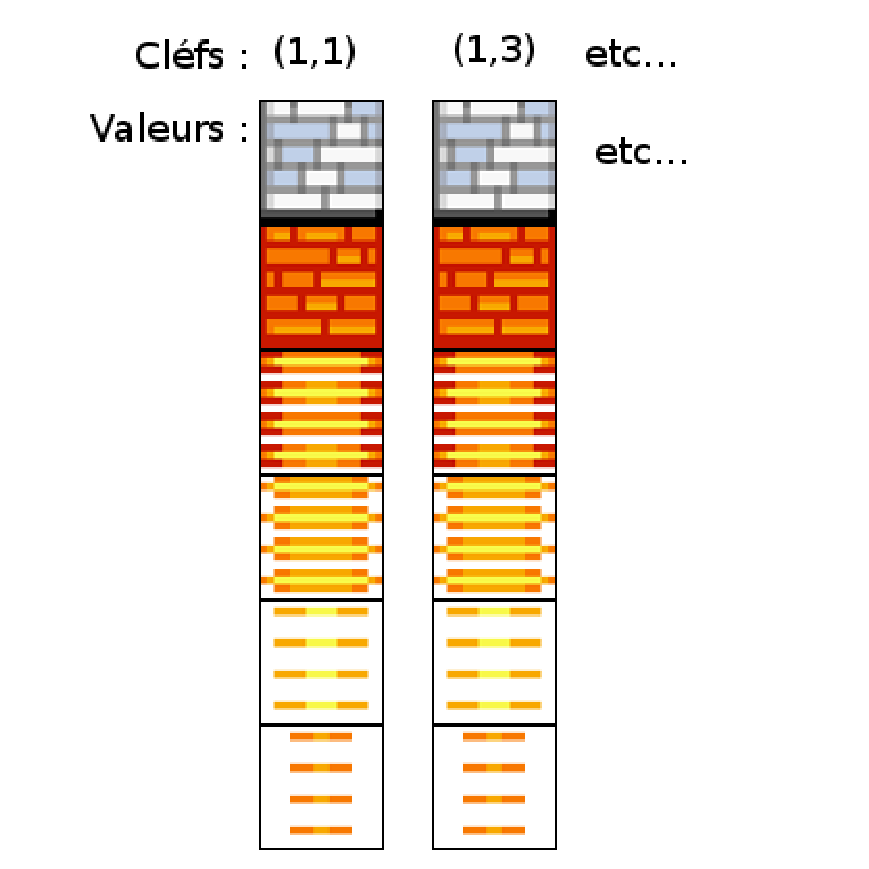
\includegraphics[width=250px, height=250px]{Developpement/Img/hashmap.eps}
					\caption{La hashmap des objets animés}
				\end{center}
			\end{figure}

			$\,$
			
			\newpage

			Les avantages d'avoir utilisé une telle structure est qu'ici au lieu de
			parcourir les 21*13*2 cases des deux matrices à chaque rafraichissement
			(c'est à dire toutes les 50 millisecondes environ) et d'afficher au minimum
			21*13 objets pour le sol et 64 objets pour les bordures si la carte est vide
			donc énormement plus si il existe d'autres objets, nous n'affichons qu'une
			image plus au maximum 197 objets.
			
			\begin{center}
				\begin{tabular}{|c|c|c|} \hline
				  & Editeur de carte & Jeu    \\\hline 
				Meilleur des cas & 337 & 1    \\\hline
				Pire des cas     & 534 & 198  \\\hline		
				\end{tabular}
			\end{center}
			
			Le meilleur des cas ici décrit une carte vide donc composée que de sol non
			animé ansi que des bordures de la carte, ce qui représente dans le nouveau
			moteur de rendu une seule et unique image contrairement à l'ancien où chaque
			objet étant affiché indépendament cela equivaut à 337 objets.
			
			$\,$
			
			Le pire des cas est une carte remplie au maximum de bloc destructibles,
			obligeant dans les deux cas à connaitre le type de sol se trouvant dessous.
			
			$\,$
			
			Nous voyons très clairement les différences de coûts entre les deux methodes
			de rendu et l'optimisation qu'engendre la deuxième.
			
			De plus ici l'utilisation de la hashmap permet dans un premier temps de
			retrouver directement un objet de par ses coordonnées mais aussi de ne pas
			avoir à parcourir $n$ cases vides comme lors de l'utilisation des matrices
			car au fur et à mesure de la partie il existera de moins en moins d'objets
			donc garder une structure aussi grosse qu'une matrice n'est pas optimal.
		
		\paragraph{Moteur physique\\}
		
			\hypertarget{Moteur physique}{}
			\label{Moteur physique}
			
			Un moteur physique est, en informatique, une bibliothèque logicielle 
			indépendante appliquée à la résolution de problèmes de la mécanique
			classique.  Les résolutions typiques sont les collisions, la chute des corps,
			les forces, la cinétique, etc.
			Les moteurs physiques sont principalement utilisés dans des simulations 
			scientifiques et dans les jeux vidéos.
			
			
			Ici notre moteur physique se contentera simplement de s'occuper des diverses
			colisions qu'auront les joueurs avec l'environnement les entourant ansi que
			les intéractions qu'auront les divers objets du décors entre eux ainsi qu'avec les joueurs.

			$\,$		
			
			Tout comme le moteur de rendu
			\footnote{
				\hyperlink{Moteur de rendu}{Moteur de rendu}
				\og voir section \ref{Moteur de rendu}, page \pageref{Moteur de rendu}.\fg
			}
			le moteur physique d'un jeu doit être optimal dans les traitements qu'il a à
			effectuer vu que son utilisation est permanente au cour du jeu.
			
			
			Afin d'optimiser ces traitements lors des collisions nous avons fusionné les
			deux matrices présentent dans l'éditeur de cartes
			\footnote{
				\hyperlink{Editeur de carte}{Editeur de carte}
				\og voir section \ref{Editeur de carte}, page \pageref{Editeur de carte}.\fg
			}
			afin de n'en obtenir qu'une seule reprenant le principe décrit dans le moteur
			de rendu\footnotemark[2].
			
			$\,$
			
			Cette matrice est composée de sept types d'objets différents à savoir :
			
			\begin{center}
				\begin{tabular}{|c|c|} \hline
				Objet  & Description \\\hline
				EMPTY  & Zone vide représentant un sol quelconque\\\hline
				BLOCK  & Un bloc \\\hline
				GAPE   & Un trou \\\hline
				DAMAGE & Une zone de dommages (piques, lasers, etc \ldots) \\\hline
				DANGEROUS\_AREA & Une zone dangereuse\\\hline
				BOMB & Une bombe\\\hline
				FIRE & Feu resultant de l'explosion d'une bombe\\\hline
				\end{tabular}
			\end{center}
			
			Les zones dangereuses sont les zones qui seront touchées lors de l'explosion
			d'une bombe, ces zones sont spécifique à l'intelligence artificielle et leur
			permettent de savoir si elles sont en danger ou non.
			
			
			$\,$
			
			Cette matrice est mise à jour lors de la pose et de l'explosion d'une bombe
			
			De cette façon il est rapide de savoir si un joueur rentre en collision avec
			un objet quelconque ou si celui-ci subit des dommages.
		

			\subparagraph{Deplacements\\}
			
				$\,$
			
				Globalement la gestion des mouvements est identique sur Android comme sur
				iOS.
				Elle consiste à poser le doigt sur l'écran et à le faire glisser dans la
				direction souhaitée ainsi le personnage avancera jusqu'à que le doigt soit
				relevé.				
				
				Quant à la gestion des colisions bien que chaque équipe utilise la matrice
				décrite ci dessus, les façons de concevoir la chose ont divergé proposant au
				final deux méthodes de rendu.
				Dans chacune le joueur se deplace verticalement, horizontalement ainsi qu'en
				diagonales.
				
				\begin{enumerate}
				  \item Colisions sous Android
				  
				  		Le principe de collisions sous Android a été de façon à faire ``glisser''
				  		ou non le joueur lorsqu'il rencontre des obstacles.
				  		
				  		
				  		Pour cela nous allons étudier un mouvement qui sera celui vers le haut
				  		afin de mieux comprendre ce terme.
				  		Nous aurions pu prendre n'importe quel aute mouvement cela serait revenu
				  		au même.
				  		
				  		Il faut juste retenir qu'au mieux le joueur est dans une case et au pire
				  		dans deux et non dans quatre car lors d'un déplacement nous n'allons
				  		regarder que la face correspondant à cette direction comme le montre
				  		l'image ci-dessous
				  		
				  		$\,$
				  		
						\begin{center}						
							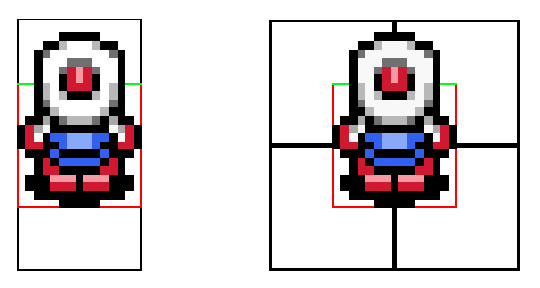
\includegraphics[width=336px,height=168px]{Developpement/Img/ex2.eps}
						\end{center}
						
				  		$\,$				  		
				  		
				  		Le trait vert représente le côté que nous étudierons lors d'un
				  		déplacement vers le haut.
				  		
				  		
				  		Nous partons du principe qu'il n'y a pas de vérification à faire tant
				  		que le joueur ne change pas de case car du moment où il y est entré
				  		c'est qu'elle est entierement traversable.
				  		
				  		Il existe donc quatres types de colisions possibles :
				  		
				  		\begin{enumerate}

				  		  \item Le premier cas correspond à celui où les cases sont
				  		  traversables, il n'y a donc qu'à déplacer le joueur vers le haut.

							\begin{center}						
								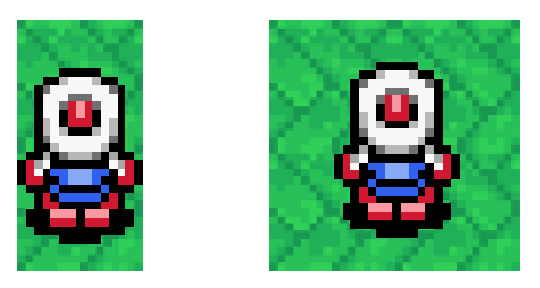
\includegraphics[width=336px,height=168px]{Developpement/Img/ok2.eps}
							\end{center}

				  		  \item Le second est celui où la ou les cases en face sont des murs, il
				  		  n'y a alors rien à faire, le personnage ne bouge pas.
				  		  				  		  
				  		  	\begin{center}						
								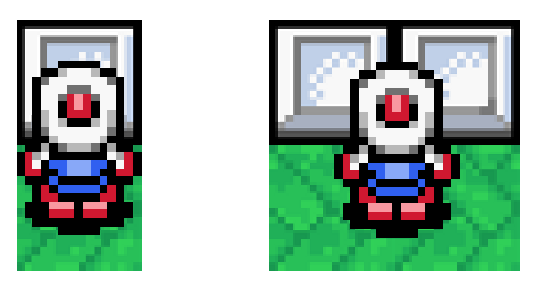
\includegraphics[width=336px,height=168px]{Developpement/Img/ko2.eps}
							\end{center}
							
				  		  \item C'est à partir de ce cas que l'on rencontre le glissement cité
				  		  plus haut.
				  		  Ici nous essayons de monter mais la case de gauche correspond à un
				  		  mur, étant donné la petitesse des écrans et la rapidité à laquelle le
				  		  jeu se déroule il serait embetant pour l'utilisateur de devoir se
				  		  decaler à droite de façon à être bien en face de la case libre.
				  		  Nous avons donc pris en compte le cas où le joueur aurait dépassé la
				  		  moitié du bloc intraversable, dans ce cas là nous le faisons glisser
				  		  sur la droite de façon à ce que celui-ci se place convenablement en
				  		  face de la case et monte normalement.
				  		  
				  		  	\begin{center}						
								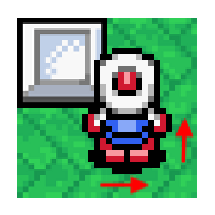
\includegraphics[width=168px,height=168px]{Developpement/Img/ko3.eps}
							\end{center}
				  		  
				  		  \item Le dernier cas est l'opposé du précédent et marche de la même
				  		  manière.
				  		  
				  		  	\begin{center}						
								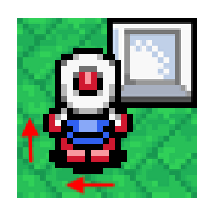
\includegraphics[width=168px,height=168px]{Developpement/Img/ko4.eps}
							\end{center}
				  		  
				  		\end{enumerate}

				  
				  \item Collisions sous iOS
				
				Le principe des collisions sous IOS a été réflechie de maniere a ce que les déplacements soit fluides et que les collisions avec des blocs ne freinnent pas la fluidité du jeu. Car en effet lors des collisions, si le joueur doit passer entre deux blocs, celui-ci doit passer au pixel pret. Cela implique que l'utilisateur doit être très minutieu dans ses déplacements et cela rend le jeu casiment injouable lors de passage entre deux blocs. Donc pour remédier à ce problème nous avons décidé d'établir un système de marge sous IOS . C'est à dire que lors de la collision avec un bloc. On va vérifier si au moin un pixel du joueur touche au moins un pixel du bloc moins une marge. Voici le tout en image:

				Il faut donc que le rectangle rouge entourant le joueur ne touche aucun autre rectangle rouge entourant les blocs pour que le joueur puisse se déplacer. Les rectangles entourant les blocs sont réduit grâce à la marge (fleche jaune) pour permettre à l'utilisateur de passer facilement.
				
				
				\end{enumerate}
			
			\subparagraph{Gestion des bombes}
				\begin{itemize}
					\item{Threads}
				\end{itemize}
	
	\subsubsection{IA}
	
		\hypertarget{IA}{}
		\label{IA}
		
		\paragraph{Pathfinding}
			\subparagraph{A*}
			\subparagraph{Aléatoire}
			\paragraph{Prise de décision}
			

	\subsubsection{Sons}
	
		\hypertarget{Sons}{}
		\label{Sons}
	
	\subsubsection{Interface utilisaeur}
		\paragraph{Android}
		\paragraph{iOS}